\newpage
\section{Social Sustainability}
Social sustainability is a frequently disregarded part of sustainability, as supportable advancement discussions frequently centre around the natural or monetary parts of supportability. In fact, all three dimensions of sustainability must be addressed to attain the most sustainable outcome possible.

Social sustainability is a process for creating sustainable and successful places that promote well-being by understanding the needs of people in the places where they live and work. Social sustainability combines the design of the physical environment with the design of the social world: infrastructure to support social and cultural life, social services, systems for engaging citizens and spaces for people and places to evolve. 

A Public Transport company like Arriva is in constant contact with its customers, whose well-being is a key aspect of the company's success. it is therefore important to assess all the aspects of social sustainability, both on the customer side but also on the internal side of the company, concerning the employees.

Having said that, we will analyze three main aspects on this topic:

\begin{itemize}
    \item Workers’ Sustainability
    \item Quality of Service
    \item Cleanliness
\end{itemize}

\subsection{Workers’ Sustainability}
Employee sustainability is the current and future ability of workers to remain in the workforce and is determined by a healthy organizational culture that supports and values employees. A sustainable employee culture keeps employees engaged to the level needed to perform their jobs capably.

Organizations that are concerned with employee sustainability recognize the need to create environments where employees remain engaged, perform at a high level, and experience job satisfaction, job commitment, and cultural buy-in throughout the duration of their employment. 

As the workforce ages, more emphasis is being placed on the importance of sustainable employment, since workers of all age groups, including those just entering the workforce, are making employee sustainability a priority in their job search.

More and more job seekers are looking to join companies that are concerned not only with environmental sustainability but are dedicated to building a culture of employee sustainability within their organizations as well.

As introduced before in \ref{sec:Intro_Innvovative}, the Sustainable Development Goals are set reach many goals at humanity level, one of which is Social Sustainability; below are listed some of the SGDs that take into account specifically the workers’ sustainability.

\begin{figure}[h!]
    \centering
    
\includegraphics[width=1\textwidth]{Images/Social_sustainability/SGD workers sustainability.PNG}
    \caption{SDGs related to Workers' Sustaibability}
    \label{fig:SDGworksus}
\end{figure}

\begin{description}
   \item[n°1 - No Poverty] According to the 1.3 SDG which aim at being able to defeat poverty, the salaries must be adjusted to the job position according to the national collective labour agreement. To monitor this aspect is useful to consider the following KPI:
   \begin{itemize}
       \item Average salary level in proportion to the national collective labour agreement
   \end{itemize}
   \item[n°4 - Quality Education ]The 4.4 SDG emphasises the importance of training education in workplace in order to have always better quality of service and to increase safety of workers and clients.
    \begin{itemize}
       \item Training hours per capita for traveling and non-traveling personnel
       \item \% Employees who received an evaluation during the year
   \end{itemize}
   \item[n°5 - Gender Equality ] In particular 5.5 SGD, prohibit any forms of discrimination and gender disparities in company employees (5.5 SDG). Some reference indicators to consider measuring the gender equity are the following:
   \begin{itemize}
       \item \% women in management area: more importance on the women full and effective participation and equal leadership opportunities at all levels of decision-making in political, economic and public life
       \item \% women with a permanent contract
       \item Ratio between training hour for woman and men
   \end{itemize}
   \item[n°8 - Decent Work and Economic Growth ] The 8 SDG remark the importance of an equal and fair salary for all workers, including young people and people with disabilities and the importance to reduce the percentage of unemployed young people who do not follow a course of study or who do not follow training courses. Going more in detail, the 8.2 SDG stresses the importance to achieve higher levels of economic productivity through diversification, technological updating and innovation, including through a focus on high value-added sectors and labour-intensive sectors. 
   \begin{itemize}
       \item \% employees with permanent contract
       \item \% employees under 35 
       \item \% turnover rate
       \item Frequency of injuries of workers
       \item Index of severity of injuries
       \item Number of hours of training on safety and health
       \item \% employees registered with trade unions
       \item Number of hours of trade union assemblies
       \item Complaints related to work practices
   \end{itemize}
   \item [n°9 - Industry, Innovation and Infrastructure ] The importance of accessing to information and communication technologies is remarked by the 9.6 SDG. In a transport company is essential to master this goal since it could provide a great amount of benefits in terms of real-time communication and feedback from the drivers on the road.
   \begin{itemize}
       \item \% Employees with company phone with application used by the company
   \end{itemize}
\end{description}

\subsection{Quality of Service}
For a long time, the performance evaluation of Public Transport (PT) has been carried out from the service managers’ perspective, based on the cost efficiency and cost effectiveness of PT services and operations. However, in the last few decades, Service Quality (SQ) has become a major area of attention for practitioners, managers and researchers, who have focused on the passengers' perspective.

The perception of Service Quality is the result of a comparison of consumer expectations with actual service performance perception or with ideal performance, depending on which type of approach we would look at. The existence of different methodologies could be justified by the complexity of the Service Quality concept, the number of attributes used to evaluate it, or the imprecision and subjectivity of the data used to analyse it, typically based on customer satisfaction surveys (CSS). 

We have considered two approaches at Service Quality in this report, one using the above cited SDGs that talk about this aspect and the other taking into account “Carta della Mobilità” of Arriva, produced every year, which is the document that regulates the relationship between PTO and the users.

\begin{figure}[h!]
    \centering
    
\includegraphics[width=0.6\textwidth]{Images/Social_sustainability/SDG service quality.PNG}
    \caption{SDGs related to Quality of Service}
    \label{fig:SDGqualiserv}
\end{figure}

\begin{description}
   \item[n°3 - Good Health and Well-Being] The 3.6 SDG has the goal to halve the number of deaths and injuries from road traffic accidents worldwide by 2020. To monitor this aspect the following KPIs can be considered: 
   \begin{itemize}
       \item Number of injuries and deaths caused by road accidents
       \item Number of road accidents
   \end{itemize}
   \item[n°5 - Gender Equality]In SDG 5.1 the main focus is to end all type of discrimination, and for our purposes we have thought of some KPIs that can be useful to monitor for a PTO on this aspect: 
    \begin{itemize}
       \item \% female passengers: this information can be collected easily if the passenger register on the website or on the application of the company 
       \item Number of assaults and violence to women on buses
   \end{itemize}
   \item[n°16 - Peace, Justice and Strong Institution ]The has the goal by 2030, to reduce illicit financing and arms trafficking, enhance the recovery and return of stolen assets and fight all forms of organized crime, reduce corruption and all its forms (16.4), Develop effective, accountable and transparent institutions at all levels (16.6). 
   
   To monitor fare evasion, corruption and arms trafficking:
    \begin{itemize}
       \item Number of passengers checked
       \item Number of clients connected on social network
       \item Number of accesses to the site
       \item Courtesy of drivers, this information is already collected with the customer satisfaction survey
       \item Number of info point in the area 
       \item Number of point of sales of tickets in the area
   \end{itemize}
\end{description}

Then, as reported in the document \textit{Carta della Mobilità}, the quality of the service can be perceived through a series of fundamental factors that characterize the quality of each aspect of the trip (e.g. travel safety, regularity of the service, cleanliness and hygienic conditions of the vehicles, etc.) and, within each of these, by specific quality indicators (for example for travel safety: number of accidents, age of vehicles) which represent the performance levels of the service provided.

Each factor and quality indicator are associated with a value (which expresses the level of quality of the service actually provided) and a target set each year by the Company providing the service.
The data on customer satisfaction are collected, in accordance with the provisions of the service contracts, with surveys carried out every six months by an external market research company through response surveys. 

Going more in detail, the surveys analyse the following aspects with their respective KPIs:

\begin{itemize}
    \item {Safety of the trip}
\begin{itemize}
    \item Accidents of the vehicles
    \item Passive accidents
    \item Age of vehicles
    \item \textit{\textbf{Total perceived safety of the trip}}
\end{itemize}
    \item Personal and property safety
    \begin{itemize}
        \item	Complaints (theft and harassment)
        \item \textit{\textbf{Total perceived personal safety}}
    \end{itemize}
    \item Regularity and punctuality of the service
    \begin{itemize}
        \item Regularity of the service
        \item Frequency of rides
        \item Commercial speed
        \item Punctuality in rush hours
        \item Punctuality in non-rush hours
        \item \textit{\textbf{Total perceived regularity of the service}}
    \end{itemize}
    \item	Comfort and cleanliness of the buses
    \begin{itemize}
        \item Crowding in rush hours 
        \item Crowding in non-rush hours 
        \item Air conditioning
        \item Low-floor bus
        \item Additional services (mobile platform, wheelchair anchoring)
        \item \textit{\textbf{Total perceived comfort}}
        \item Ordinary cleaning
        \item Extraordinary cleaning
        \item Cleaning of bus stations
        \item \textit{\textbf{Total perceived cleanliness}}
    \end{itemize}
    \item Information and service to users
    \begin{itemize}
        \item Timeliness
        \item Internal visual devices
        \item Timetable at bus stops
        \item Point of sales of tickets
        \item Feedback to complaints
        \item \textit{\textbf{Total perceived information and services}}
    \end{itemize}
    \item Relational aspects
        \begin{itemize}
            \item  \textit{\textbf{Total perceived relational aspects}}
        \end{itemize}
    \item Attention to environment
        \begin{itemize}
            \item Electric or hybrid vehicles 
            \item Use of eco-fuels
            \item Vehicles Euro 3-4
            \item Vehicles Euro 4 and more
            \item \textit{\textbf{Total perceived attention to environment}}
        \end{itemize}
\end{itemize}

The KPIs are reported in the following graph, with a range value of [0,4]; as we can see, in 2019 there was an improvement in all indicators, except for the perceived security. For the year 2020 the data are not available because the surveys were not carried out due to the Covid pandemic.

\begin{figure}[h!]
    \centering
    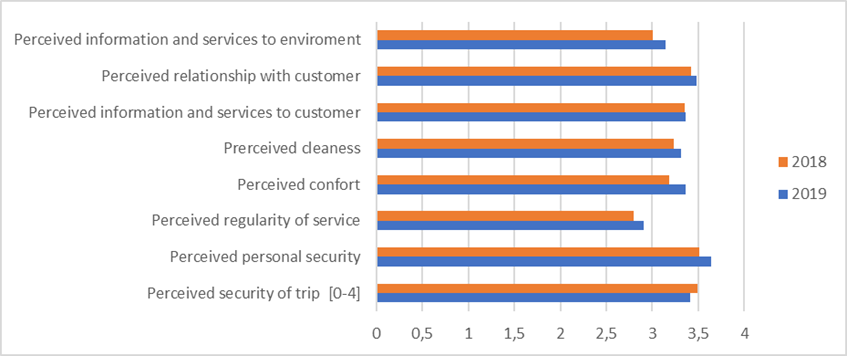
\includegraphics[width=0.9\textwidth]{Images/Social_sustainability/graph.png}
    \caption{Summary KPIs related to "Carta della Mobilità" document}
    \label{fig:kpiscdm}
\end{figure}

\subsection{Cleanliness}
Since we are living in a very particular historic period where an excellent quality of sanitary conditions is essential, we wanted to deepen the aspect of Bus Cleanliness, already partially assessed in the chapter above.

Our interest was confirmed by the fact that cleaning requirements by the PTA has changed and become stricter. The importance of the cleaning is confirmed in the service contract, which establishes penalties in case of:
\begin{itemize}
    \item failure to comply the frequency and/ or cycles in relation to the individual types of intervention (both for ordinary and extraordinary cleaning of the fleet and infrastructure and network systems open to the public)
    \item Insufficient cleaning of the bus (both for ordinary and extraordinary cleaning of the fleet and infrastructure and network systems open to the public)
\end{itemize}

The main requirements for cleanliness in today's PTA are:

\begin{itemize}
    \item daily cleaning (ordinary cleaning): it consists of removing the filth produced by the passengers, cleaning of cockpit, floor and handrails (about 10-15 min per bus)
    \item monthly cleaning (extraordinary cleaning): it is a deeper cleaning; special products must be used to remove dirt (generally it takes at least 30-40 min per bus)
    \item half yearly cleaning: vehicles are subjected to an antibacterial sanitization and disinfestation cycle 
\end{itemize}

Nowadays, due to the pandemic situation, the consortium has introduced from March 2020 sanitation interventions with disinfection and sanitization in particular of the surfaces and passenger support points. Also, every fifteen days during the periodic cleaning interventions are performed cleaning by ionization

\subsection{Mock Up Dashboard}
As per the previous chapter \ref{sec:newtech}, the aim of this is to built and visualize some mock-up dashboard pages, starting from the KPIs listed above in the previous paragraphs.

Also for this section, all pages are a mock-up also for what concerns the data present in he graphs, which may appear not close to the reality and made on purpose to talk about their benefits.

\newpage

\newpage
\begin{landscape}
\thispagestyle{empty}
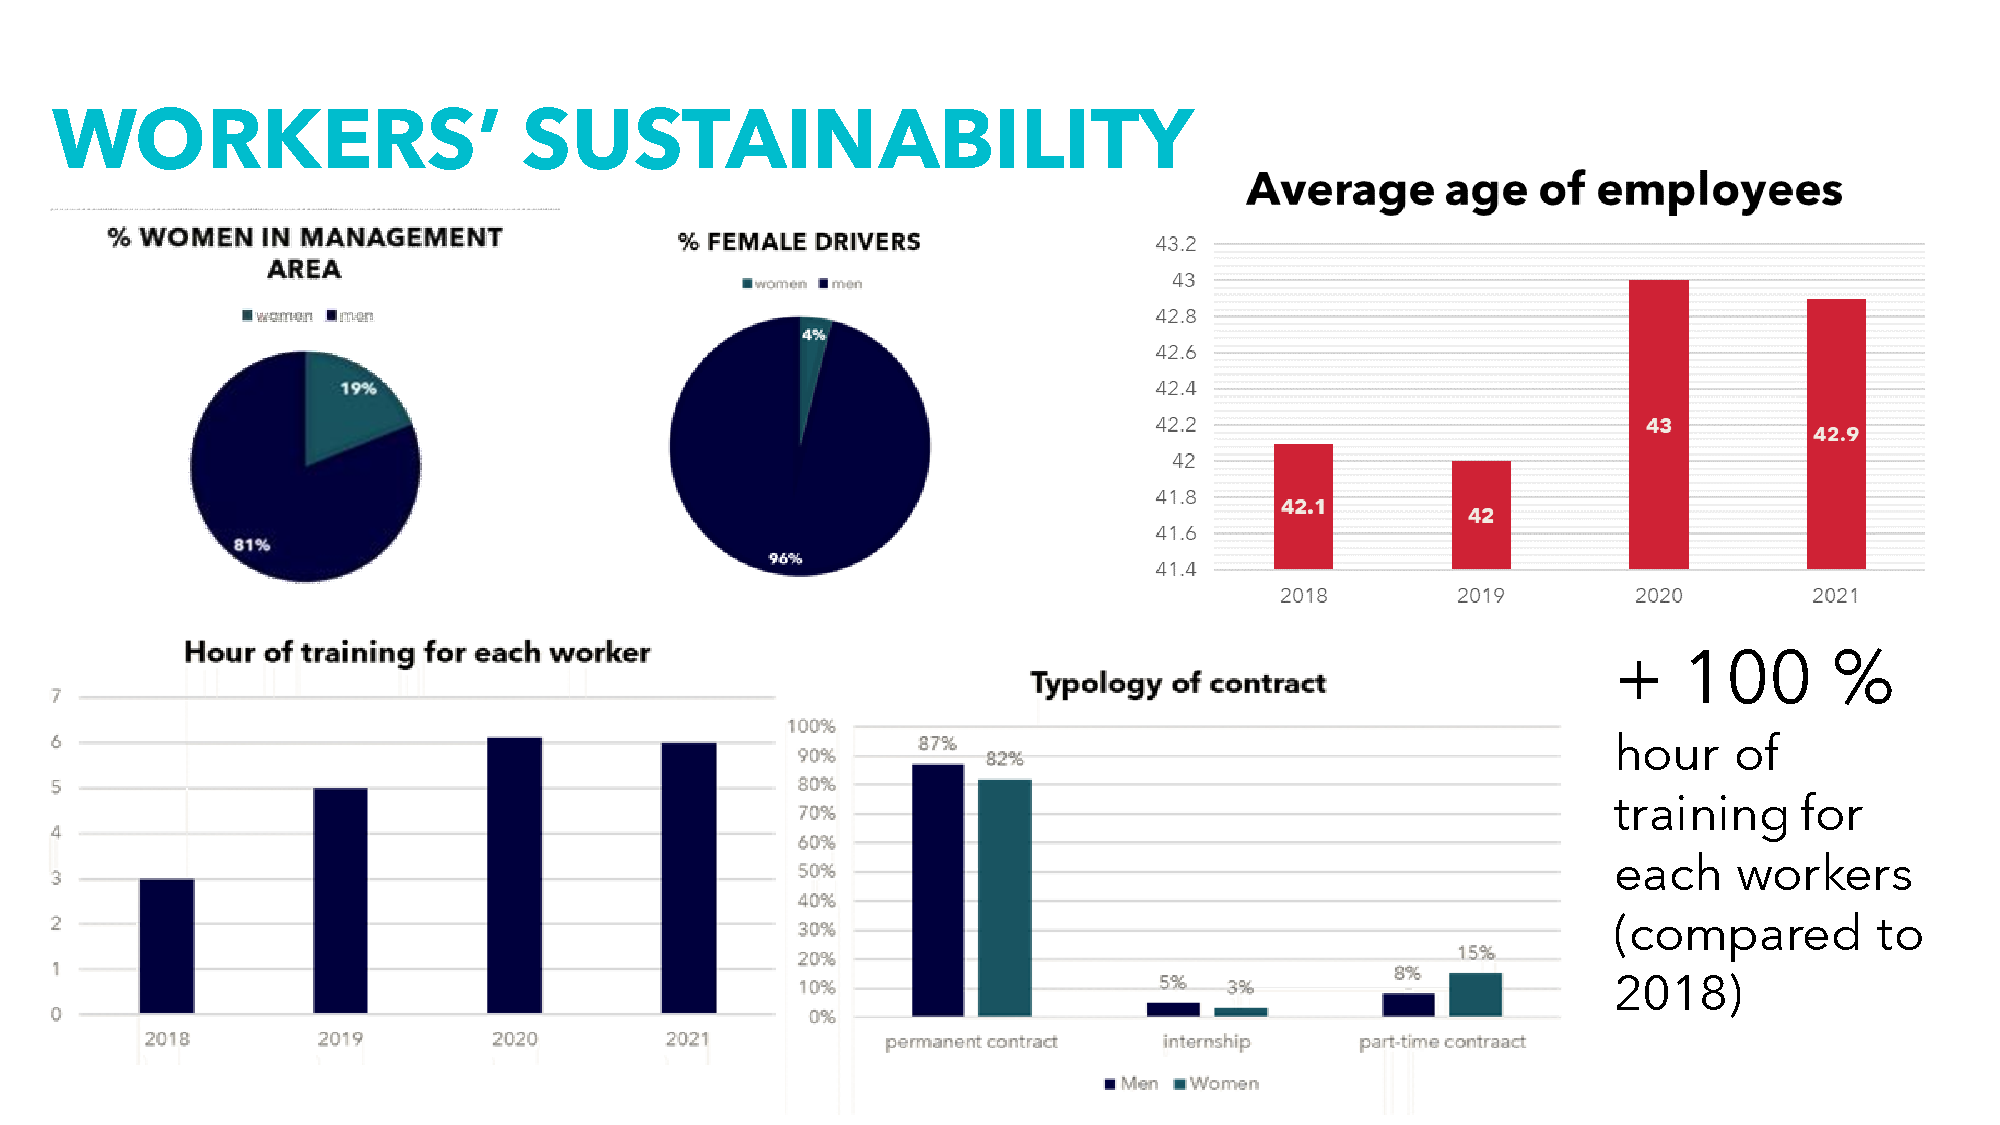
\includepdf[angle=90, pagecommand={\null\enlargethispage{3\baselineskip}\vfill\captionof{figure}{Workers' Sustainability page}\label{fig:work2}}]{mockup/workers.pdf}
\end{landscape}

\subsubsection{Workers' Sustainability}
The dashboard shows the main features of workers sustainability. All the data necessary to build this type of dashboard are already available within the company and do not risk additional technologies.In order to guarantee equal treatment between men and women also in the workplace, it is also necessary to know the proportion of men and women both in the managerial area and among the traveling staff.
another indicator to monitor inequalities is the type of contract offered to men and women (permanent contract, internship, part-time contract).
Safety is also essential in the workplace. to safeguard workers' lives, in addition to strict controls on safety provisions, it is also necessary to inform and train staff. For this reason, the dashboard shows the number of hours of training followed on average by each worker. For the various indicators a trend is reported from 2018 to 2021 in order to see the improvements, as in this case, or to be able to find the critical issues and solve them.

\newpage
\begin{landscape}
\thispagestyle{empty}
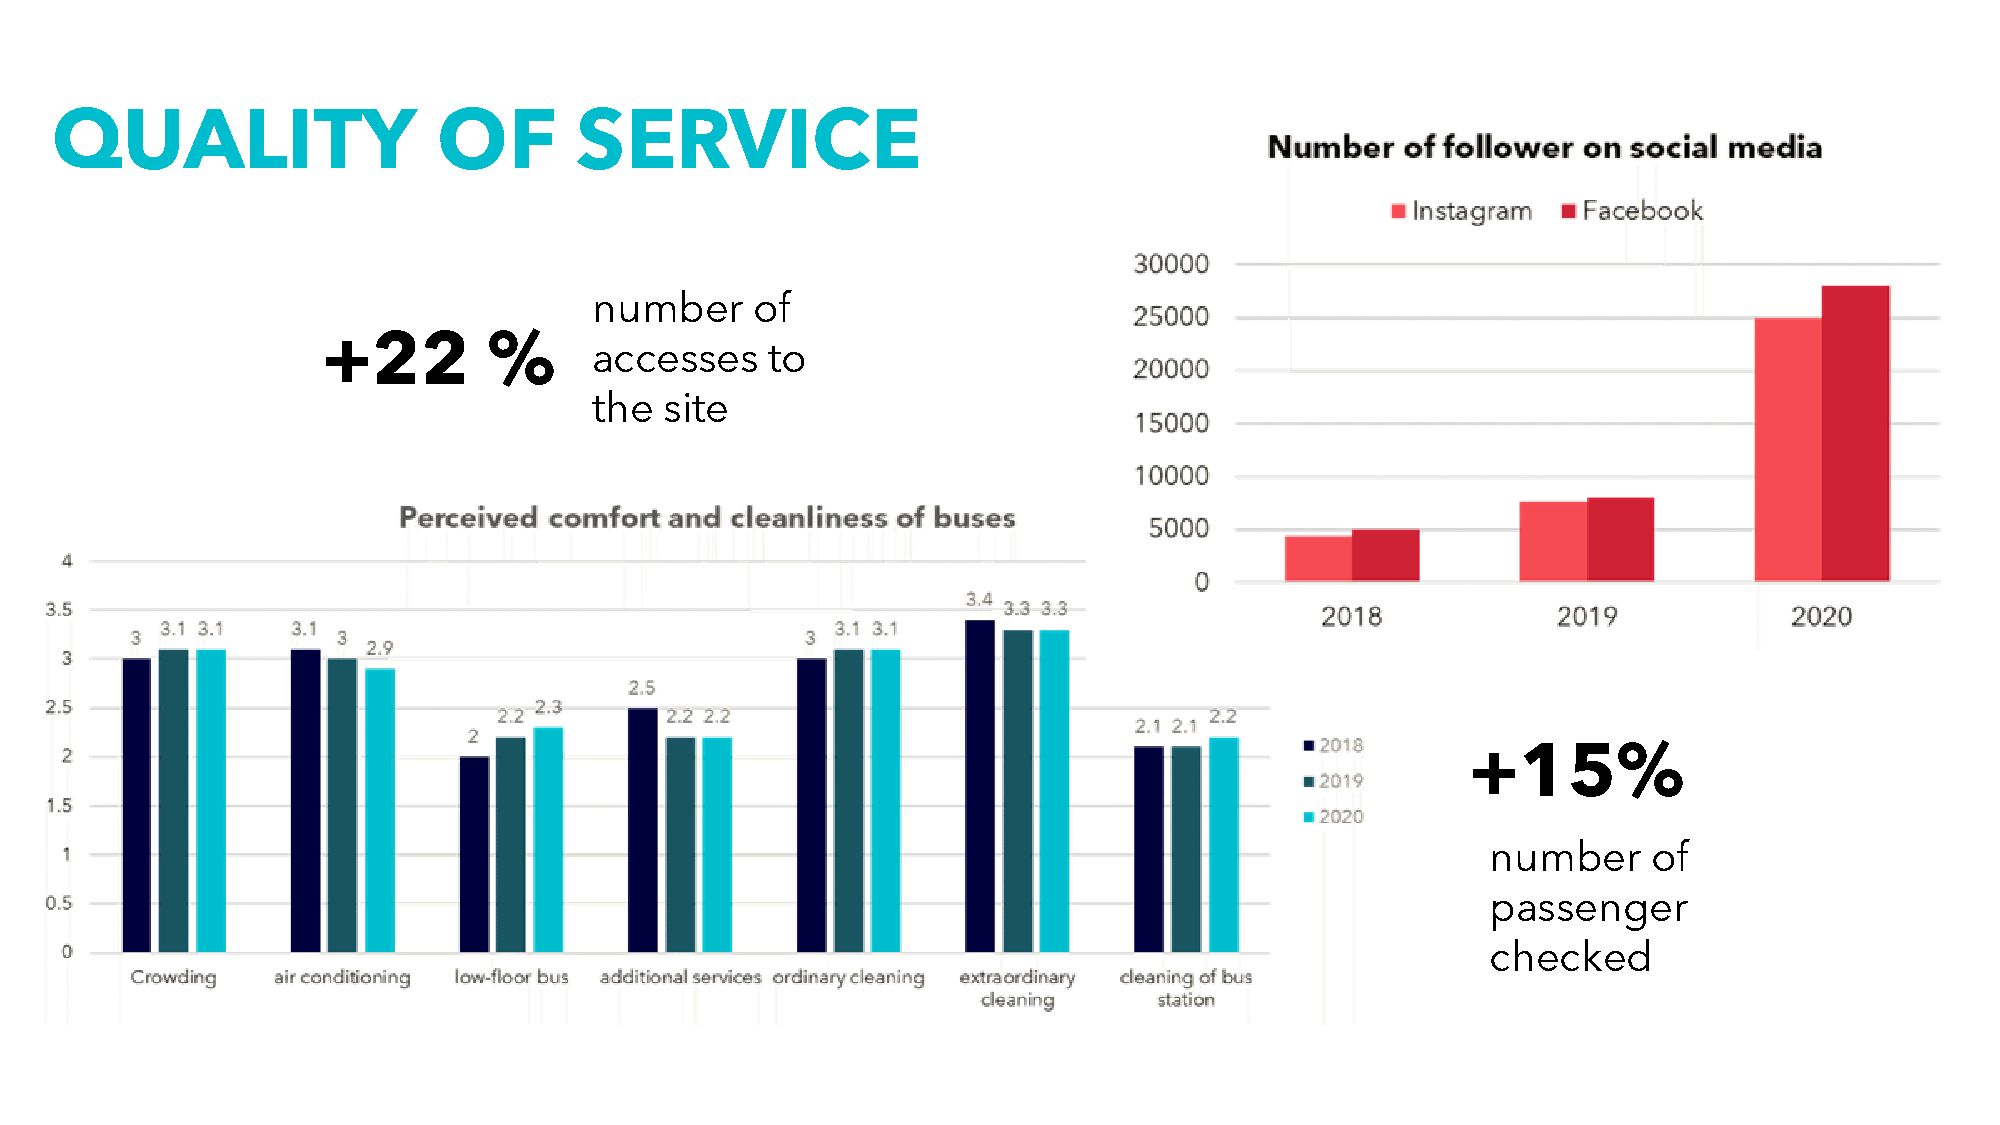
\includepdf[angle=90, pagecommand={\null\enlargethispage{3\baselineskip}\vfill\captionof{figure}{Quality of Service page}\label{fig:qs}}]{mockup/qualitysocial.pdf}
\end{landscape}

\subsubsection{Quality of Service}
The data regarding the quality of the service are collected through an annual questionnaire and are therefore already available. the dashboard in particular shows the parameter concerning the comfort and cleanliness at the edge of the vehicles. it is important to note how this parameter has changed over the years and also to break down this parameter to see what are the aspects on which it is possible to improve. furthermore, through the new technologies presented above, such as the people counter, a more objective value can be given to the parameter concerning the crowding of vehicles.

At the bottom of the dashboard some data are provided regarding the number of people registered on the company's social channels and the number of applications or accesses to the official website. these aspects of the service, considered in the past less important, are useful because they are closely related to both customer loyalty and fare evasion




